\subsubsection{Organization chart orientation
\label{sec:org-chart-orientation}}

A common method of describing relations within the bureaucracy is the organization chart (colloquially, the ``\gls{org chart}"). \iftoggle{glossaryinmargin}{\marginpar{[Glossary]}}{}
Normally the Chief Executive Officer (CEO) is at the top of the chart, middle management is in the middle, and managed employees are at the bottom. See figure~\ref{fig:org_chart_orientation_ceo-at-top}\iftoggle{haspagenumbers}{ on page~\pageref{fig:org_chart_orientation_ceo-at-top}.}{.}

Artifacts like org charts subtly convey an organization's culture. 
% What's the point of this section? Is there a consequence, or is this just an observation?
There are emotional connotations to alternative layouts. You can alter expected relations (culture and norms) by playing with the orientation of the org chart.
Org chart orientation can be overanalyzed, so this exploration is limited.

The point of thinking about org chart orientation is to frame how you perceive your supervisors, peers, and subordinates. Notice that the framing is embedded in the words -- prefixes super (over) and sub (under). 
These concepts inform what you expect from relations.
Do I seek support or direction and guidance from my boss? What do I expect from my boss? My peers? My subordinates? What do I expect to provide them?

%\begin{itemize}
%\item 
%\end{itemize}

The relative orientation of the \href{https://en.wikipedia.org/wiki/Chief_executive_officer}{CEO} 
\index{Wikipedia!Chief Executive Officer@\href{https://en.wikipedia.org/wiki/Chief_executive_officer}{Chief Executive Officer}}\iftoggle{WPinmargin}{\marginpar{$>$Wikipedia: CEO}}{}
to the workers sets expectations for relations. 
Options for orientation are the conventional CEO at top
(figure~\ref{fig:org_chart_orientation_ceo-at-top}), 
CEO at the bottom (figure~\ref{fig:org_chart_orientation_ceo-at-bottom}),
CEO on the right (figure~\ref{fig:org_chart_orientation_ceo-leads}),
CEO on the left (figure~\ref{fig:org_chart_orientation_ceo-follows}),
CEO as the center of a star 
(for example, the \href{https://en.wikipedia.org/wiki/File:League_of_Nations_Organization.png}{League of Nations diagram}.)
\index{Wikipedia!League of Nations diagram@\href{https://en.wikipedia.org/wiki/File:League_of_Nations_Organization.png}{League of Nations diagram}}

\begin{figure}
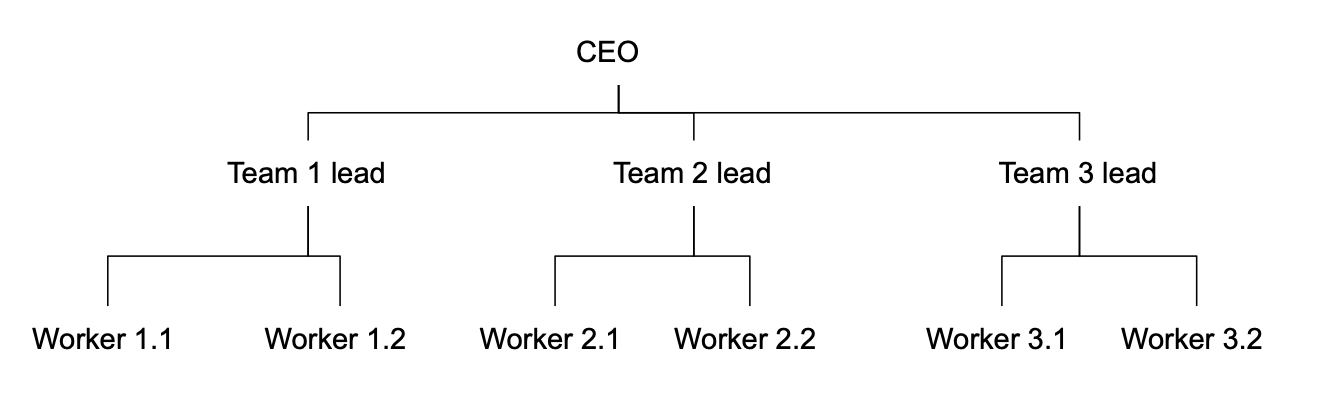
\includegraphics[width=1\textwidth]{images/org-chart-orientation-ceo-at-top.pdf}
\caption{Standard orientation. The role with the most responsibility and authority is at the top. Left-right ordering is intended to be irrelevant in this view, though left-to-right reading order emphasizes importance.}
\label{fig:org_chart_orientation_ceo-at-top}
\end{figure}

\begin{figure}
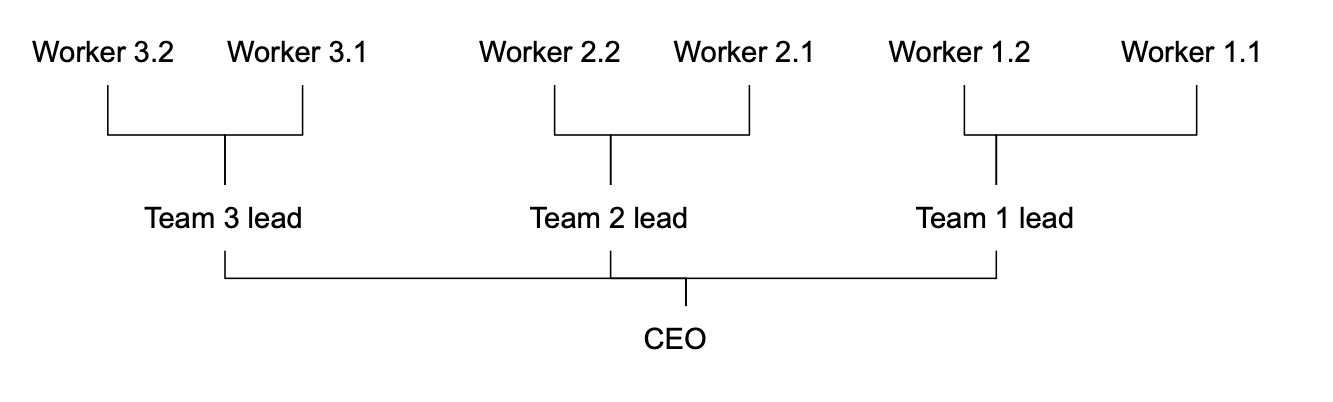
\includegraphics[width=1\textwidth]{images/org-chart-orientation-ceo-at-bottom.pdf}
\caption{Flipping the orientation presents a more realistic view of the CEO's responsibility. The crushing burden of servant leadership is clear. Left-right ordering is intended to be irrelevant in this view.}
\label{fig:org_chart_orientation_ceo-at-bottom}
\end{figure}

\begin{figure}
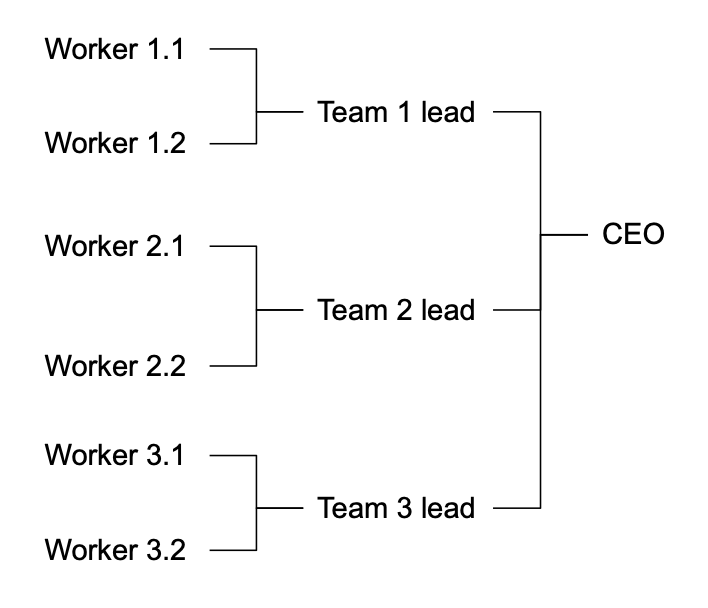
\includegraphics[width=0.8\textwidth]{images/org-chart-orientation-ceo-leads.pdf}
\caption{Conventionally time flows from left (old) to right (new), so in this graph the CEO leads the charge into the unknown. Is the CEO dragging workers forward, or are the workers pushing the CEO? The top-to-bottom order can be read as importance. }
\label{fig:org_chart_orientation_ceo-leads}
\end{figure}

\begin{figure}
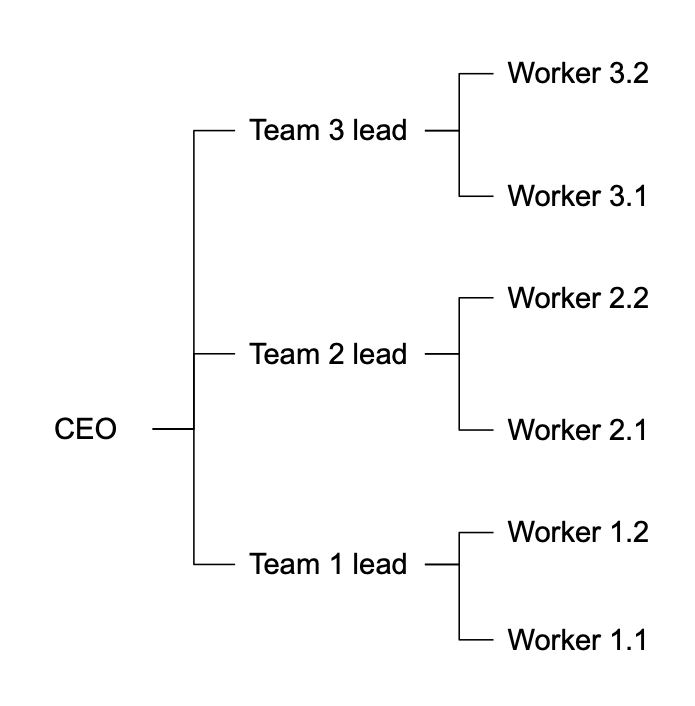
\includegraphics[width=0.8\textwidth]{images/org-chart-orientation-workers-lead.pdf}
\caption{The ``chariot view'' with the CEO in the chariot and the workers out front. Workers are in the future; the CEO is in the past operating on old information. As with figure~\ref{fig:org_chart_orientation_ceo-leads}, top-to-bottom ordering can be read as importance. }
\label{fig:org_chart_orientation_ceo-follows}
\end{figure}

\begin{figure}
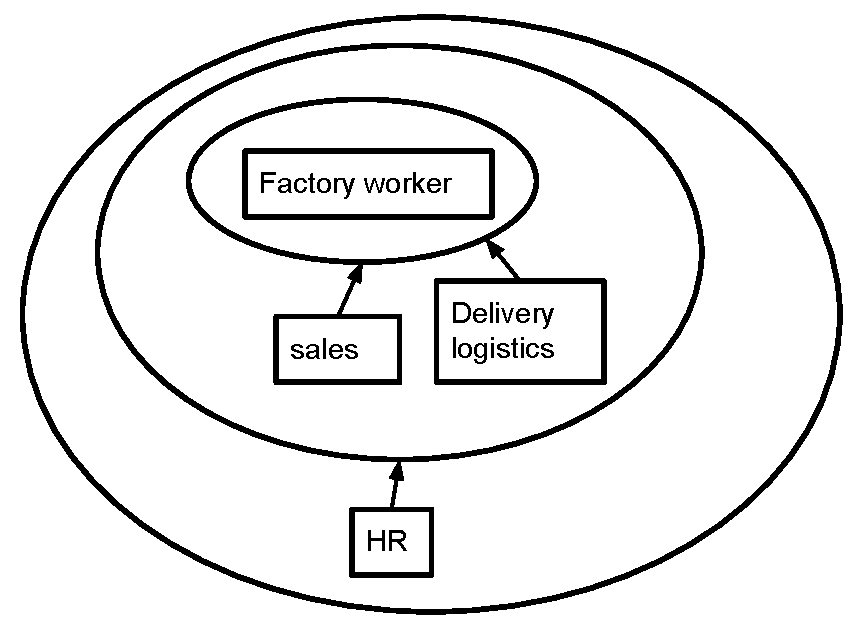
\includegraphics[width=0.8\textwidth]{images/org_chart_wedding_cake_dependencies_-_manufacturing.pdf}
\caption{A dependency-oriented view rather than a reporting-oriented view. The center of the bullseye is the team that generates the value that is the focus of the business or the organization.
The outer rings support teams that exist in the inner rings. The diagram is specific to an organization's domain. This visualization identifies which teams are the customers of which other teams in an organization.}
\label{fig:org_chart_wedding_cake_manufacturing}
\end{figure}



%extension of 
% \href{https://en.wikipedia.org/wiki/Conway\%27s_law}{Conway's law}: seating chart reflects org chart